\chapter{Introduction}

\subsubsection{What is \khepera{}}
The \khepera{} is a small differential wheeled robot (diameter of 5.5cm). 
It has eleven infrared sensors, nine around it and two on the bottom. 
Additionally, it has five ultrasonic sensors around it. It can communicate 
with Bluetooth and is equipped with a battery that provides him 
approximately four hours of autonomy. There is a commercialized device 
called KoreBot II that can provide the \khepera{} limited computing 
capacity. 

\subsubsection{Kind of research that will make use of it}
As the research in the lab is directed toward expensive machine learning 
algorithms, the limited computing capacity of the KoreBot II was not 
interesting. It would be more efficient to use the computing power of 
a dedicated computer and communicate with the \khepera{} through 
Bluetooth.

The actual researches of Manuel Blum do not explicitly concern problems 
of mobile robotics. Thus, it has been decided that the first environment 
in which the \khepera{} will evolve would not make use of the sensors, 
but of an external detector that keeps track of the robot position and 
orientation. The main idea is simply to solve a physical problem based 
on the knowledge gained from a virtual training on this problem, in 
other words, from a simulation.

\subsubsection{Classical maze problem}
The \clsquare{} system already includes a maze plant where it is possible 
to solve the shortest-path problem from a given position to a given 
target. As I concentrated on building the modules needed to detect and 
pilot the \khepera{}, I used this plant so I do not have to worry 
about the problem itself (solving a maze).

In a first time, I built a module to detect the position and the 
orientation of the \khepera{} with the help of a camera hanging from 
the ceiling above the maze. In a second time, I created a navigation 
system for the robot with the help of the position detector. In a 
last step, I built a module to get a virtual discretized description 
of a physical maze. I finally linked the detectors with the maze plant 
that I customized a little bit.
\\
\\
In the first chapter of this document, I will explain the modules built 
for the detectors inside of the Tapir system. In the second chapter, 
I will explain every classes and modules I had to build for the \clsquare{}.
Then in the third chapter, I will explain how to set up and run an 
experiment with the \khepera{} and a maze using the tools explained 
in previous chapters. 

\begin{figure}
    \begin{center}
        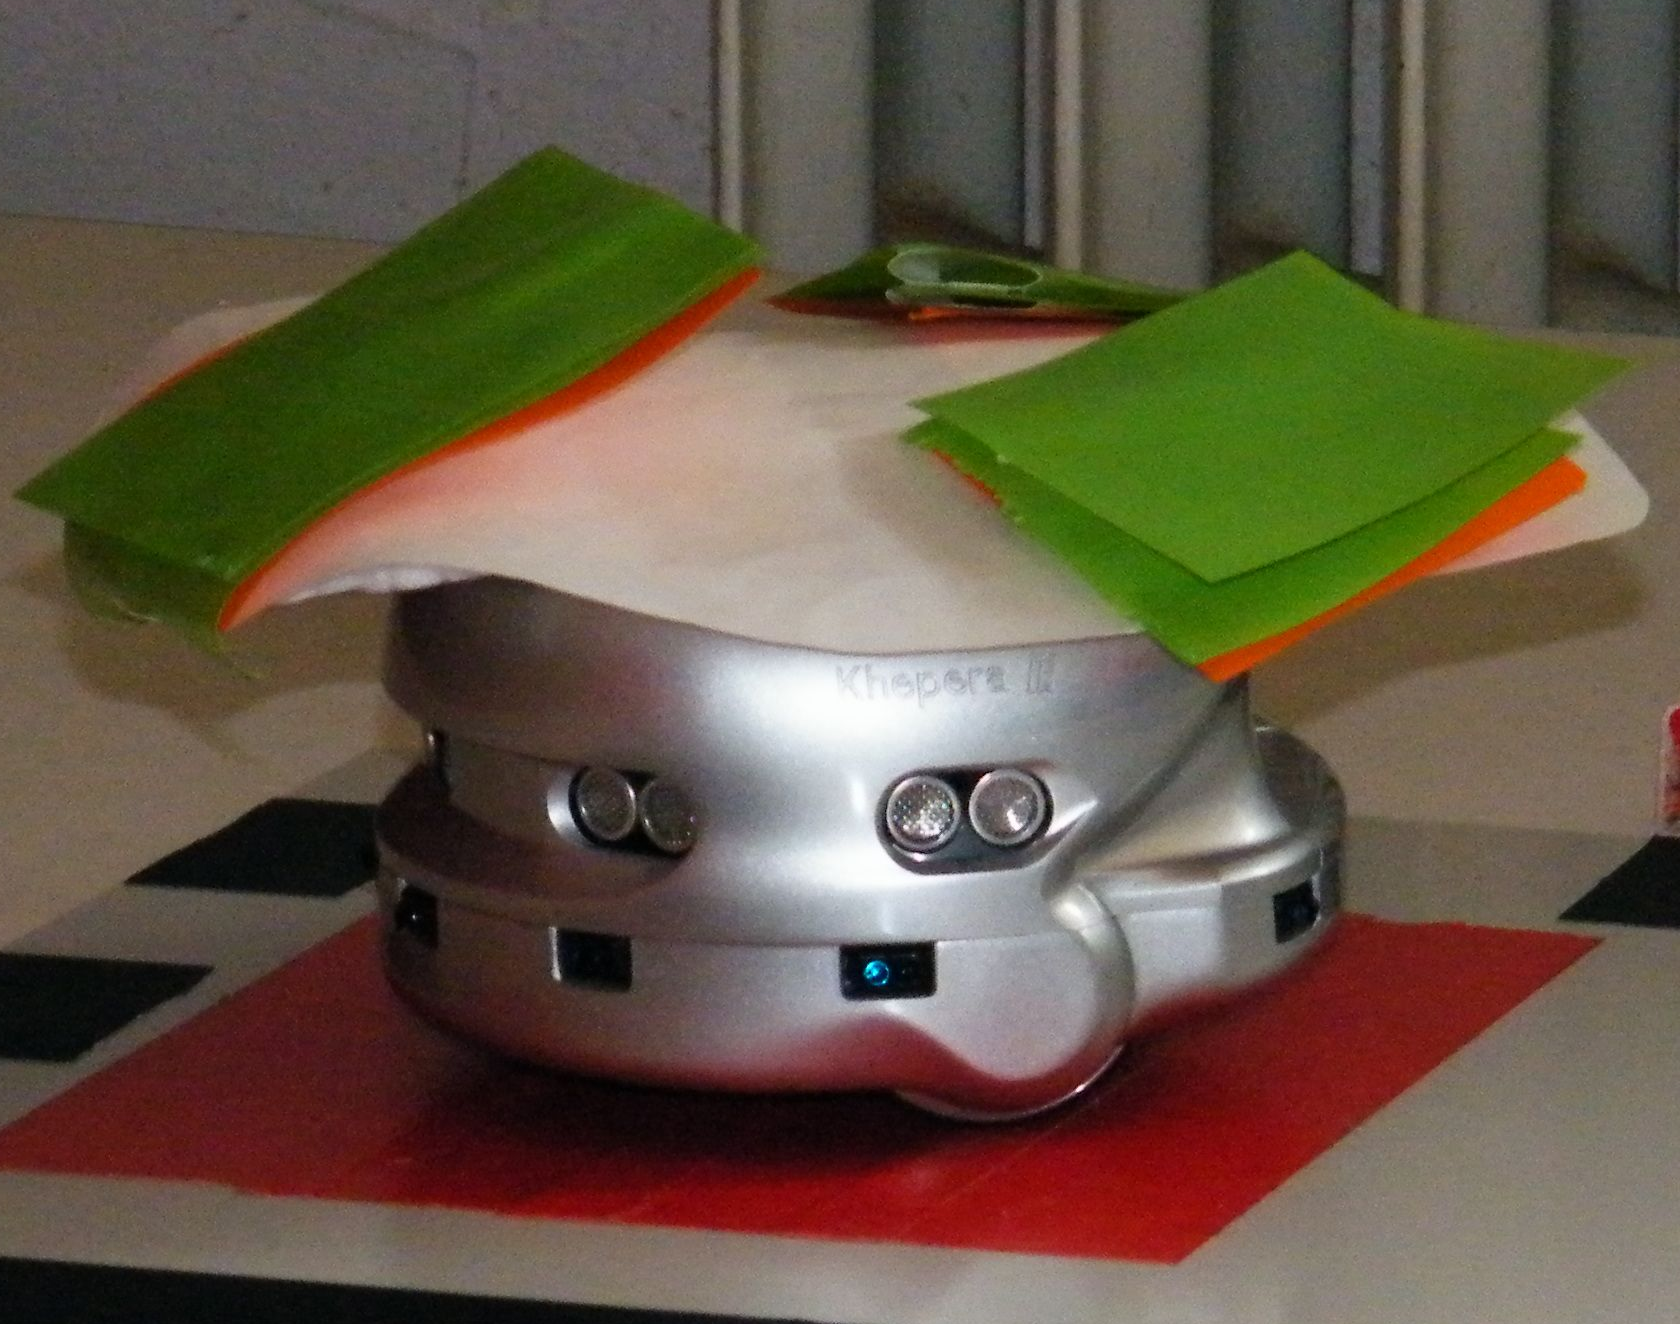
\includegraphics[width=\textwidth]{./img/kheperacrop.png}
        \caption[The \khepera{}]{%
        The \khepera{} with his little hat for detection}
    \end{center}
\end{figure}
